\documentclass[aspectratio=169,11pt]{beamer}
\usepackage[T1]{fontenc}
\usepackage{lmodern}
\usepackage{amsmath,amssymb,mathtools}
\usepackage{tikz}
\usetikzlibrary{arrows.meta,positioning,calc,fit,backgrounds,shapes.geometric,decorations.pathreplacing}
\usepackage{booktabs}
\usepackage{xcolor}

\definecolor{mainblue}{RGB}{26,64,133}
\definecolor{accent}{RGB}{176,86,20}
\definecolor{softblue}{RGB}{232,239,250}
\definecolor{softgrey}{RGB}{243,243,243}

\usetheme{Boadilla}
\setbeamertemplate{navigation symbols}{}
\setbeamercolor{structure}{fg=mainblue}
\setbeamercolor{frametitle}{bg=mainblue!10,fg=mainblue}
\setbeamercolor{title}{fg=mainblue}
\setbeamercolor{author}{fg=black!70}
\setbeamertemplate{itemize items}[circle]
\setbeamertemplate{blocks}[rounded][shadow=false]
\setbeamerfont{frametitle}{size=\large,series=\bfseries}

\newcommand{\abs}[1]{\lvert #1\rvert}
\newcommand{\R}{\mathbb R}
\DeclareMathOperator{\rank}{rank}
\DeclareMathOperator{\im}{im}

% takeaway strip at the bottom of a frame
\newcommand{\takeaway}[1]{%
  \vfill
  \begin{beamercolorbox}[wd=\dimexpr\textwidth-9pt\relax,sep=4pt,rounded=true]{block body}
    \footnotesize\color{mainblue}\textbf{Takeaway.} \color{black}#1
  \end{beamercolorbox}}

\title[Seymour's second-neighborhood conjecture]{A proof of Seymour's second-neighborhood conjecture}
\subtitle{after OpenAI's preprint; a guided tour of the proof}
\author{}
\date{}

\begin{document}

\begin{frame}
  \titlepage
  \begin{center}\footnotesize\color{black!60}
    one conjecture, three engines, one contradiction
  \end{center}
\end{frame}

\begin{frame}{The conjecture}
  \begin{columns}[T]
  \begin{column}{0.50\textwidth}
    \small
    An \emph{oriented graph}: no loops, no two arcs the same way, never both $x\to y$ and $y\to x$.
    \medskip

    For a vertex $v$:
    \[
      N_1^+(v)=\{u:\ v\to u\},
    \]
    \[
      N_2^+(v)=\bigl\{w\notin\{v\}\cup N_1^+(v): \exists u,\ v\to u\to w\bigr\}.
    \]
    \medskip
    \textbf{Conjecture (Seymour; Dean--Latka).} Some $v$ has
    $\abs{N_1^+(v)}\le\abs{N_2^+(v)}$.
  \end{column}
  \begin{column}{0.48\textwidth}
    \centering
    \scalebox{0.78}{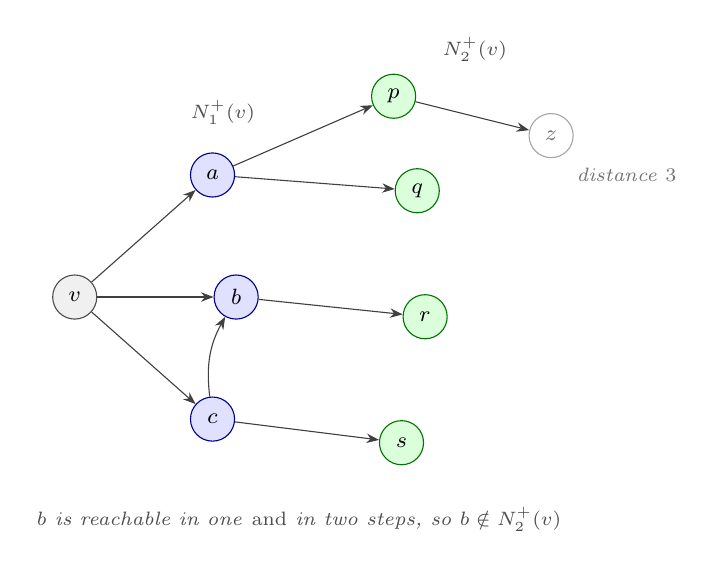
\begin{tikzpicture}[
  vertex/.style={circle,draw=black!70,fill=black!6,inner sep=0pt,minimum size=5.6mm,
                 font=\footnotesize},
  first/.style={circle,draw=blue!55!black,fill=blue!12,inner sep=0pt,minimum size=5.6mm,
                font=\footnotesize},
  second/.style={circle,draw=green!45!black,fill=green!14,inner sep=0pt,minimum size=5.6mm,
                 font=\footnotesize},
  far/.style={circle,draw=black!35,fill=white,inner sep=0pt,minimum size=5.6mm,
              font=\footnotesize,text=black!55},
  arc/.style={-{Stealth[length=1.6mm]},draw=black!75},
  lab/.style={font=\scriptsize\itshape,text=black!70}
]
% vertices
\node[vertex] (v) at (0,0) {$v$};
\node[first]  (a) at (1.75,1.55) {$a$};
\node[first]  (b) at (2.05,0)    {$b$};
\node[first]  (c) at (1.75,-1.55){$c$};
\node[second] (p) at (4.05,2.55) {$p$};
\node[second] (q) at (4.35,1.35) {$q$};
\node[second] (r) at (4.45,-0.25){$r$};
\node[second] (s) at (4.15,-1.85){$s$};
\node[far]    (z) at (6.05,2.05) {$z$};
% arcs
\draw[arc] (v) -- (a);
\draw[arc] (v) -- (b);
\draw[arc] (v) -- (c);
\draw[arc] (a) -- (p);
\draw[arc] (a) -- (q);
\draw[arc] (b) -- (r);
\draw[arc] (c) -- (s);
\draw[arc] (c) to[bend left=18] (b);
\draw[arc] (p) -- (z);
% region labels (placed clear of every node and arc)
\node[lab,anchor=west] at (1.35,2.35) {$N_1^+(v)$};
\node[lab,anchor=west] at (4.55,3.15) {$N_2^+(v)$};
\node[lab,anchor=west,text=black!55] at (6.25,1.55) {distance $3$};
\node[lab,anchor=north] at (2.85,-2.55) {$b$ is reachable in one \emph{and} in two steps,
                                        so $b\notin N_2^+(v)$};
\end{tikzpicture}
}
  \end{column}
  \end{columns}
  \takeaway{The two neighborhoods are disjoint, and ``distance two'' is \emph{exact}:
  the vertex $b$ of the picture is in $N_1^+$ and reachable in two steps, so it is not in $N_2^+$.}
\end{frame}

\begin{frame}{Why this is not obvious}
  \small
  \begin{itemize}
    \item A \emph{tournament} (an arc between every two vertices): Dean's conjecture, proved by
      Fisher 1996, again by Havet--Thomass\'e 2000.
    \item General oriented graphs: known only with degree hypotheses, or up to a ratio
      $\abs{N_2}/\abs{N_1}\approx0.7155$ (Huang--Peng 2024).
    \item Every vertex can have more out-neighbors than second out-neighbors? Then no
      minimality, no greedy choice, and no local move is available: deleting a vertex changes
      everybody's neighborhoods.
    \item A sink satisfies the conclusion trivially ($0\le0$), so the whole difficulty is in
      graphs where every vertex has an in-neighbor.
  \end{itemize}
  \takeaway{We must prove something about \emph{all} vertices at once, so the proof is a global
  argument, not a search for a good vertex.}
\end{frame}

\begin{frame}{Main theorem}
  \begin{block}{Theorem}
    Every nonempty finite oriented graph has a vertex $v$ with
    $\abs{N_1^+(v)}\le\abs{N_2^+(v)}$.
  \end{block}
  \medskip
  \small
  Two consequences follow (and are not used in the proof):
  \begin{itemize}
    \item the vertex- and arc-weighted forms, via Seacrest's equivalences;
    \item minimum in- and out-degree $\ge n/3$ forces a directed triangle; a regular oriented
      graph of directed girth $4$ has $n\ge 3r+1$.
  \end{itemize}
  \takeaway{The statement needs no hypothesis at all; the proof nevertheless forces
  ``positive indegree'' on the object it studies.}
\end{frame}

\begin{frame}{The shape of the proof}
  \centering
  \scalebox{0.76}{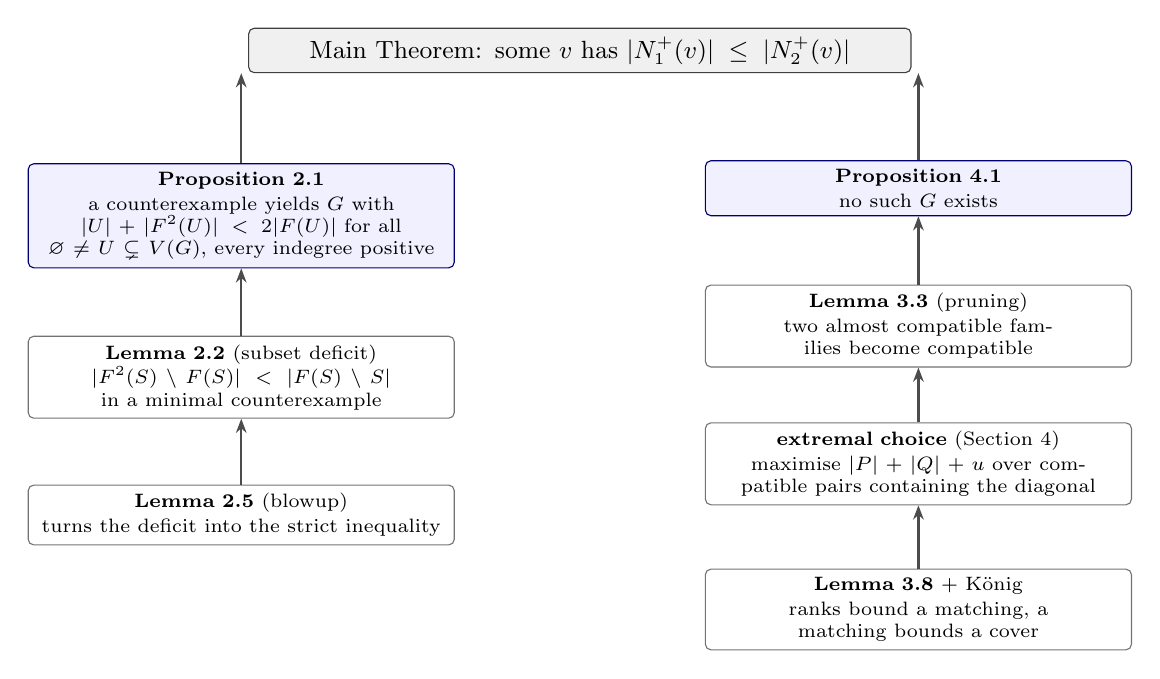
\begin{tikzpicture}[
  box/.style={draw=black!55,fill=white,rounded corners=2pt,align=center,
              font=\scriptsize,inner sep=3pt,text width=#1},
  box/.default=5.2cm,
  thm/.style={box=8.2cm,draw=black!75,fill=black!6,font=\small},
  ar/.style={-{Stealth[length=1.8mm]},draw=black!70,thick}
]
\node[thm] (T) at (0,0) {Main Theorem: some $v$ has $\abs{N_1^+(v)}\le\abs{N_2^+(v)}$};
\node[box,draw=blue!45!black,fill=blue!6] (P2) at (-4.3,-2.1)
  {\textbf{Proposition 2.1}\\[1pt] a counterexample yields $G$ with
   $\abs{U}+\abs{F^2(U)}<2\abs{F(U)}$ for all $\varnothing\ne U\subsetneq V(G)$,
   every indegree positive};
\node[box,draw=blue!45!black,fill=blue!6] (P4) at (4.3,-1.75)
  {\textbf{Proposition 4.1}\\[1pt] no such $G$ exists};
\node[box] (L22) at (-4.3,-4.15)
  {\textbf{Lemma 2.2} (subset deficit)\\[1pt]
   $\abs{F^2(S)\setminus F(S)}<\abs{F(S)\setminus S}$ in a minimal counterexample};
\node[box] (L23) at (-4.3,-5.9)
  {\textbf{Lemma 2.5} (blowup)\\[1pt] turns the deficit into the strict inequality};
\node[box] (L31) at (4.3,-3.5)
  {\textbf{Lemma 3.3} (pruning)\\[1pt] two almost compatible families become compatible};
\node[box] (EX) at (4.3,-5.25)
  {\textbf{extremal choice} (Section 4)\\[1pt] maximise $\abs P+\abs Q+u$ over compatible
   pairs containing the diagonal};
\node[box] (L32) at (4.3,-7.1)
  {\textbf{Lemma 3.8} + K\"onig\\[1pt] ranks bound a matching, a matching bounds a cover};
\draw[ar] (P2.north) -- (T.south -| P2.north);
\draw[ar] (P4.north) -- (T.south -| P4.north);
\draw[ar] (L22.north) -- (P2.south);
\draw[ar] (L23.north) -- (L22.south);
\draw[ar] (L31.north) -- (P4.south);
\draw[ar] (EX.north) -- (L31.south);
\draw[ar] (L32.north) -- (EX.south);
\end{tikzpicture}
}
  \takeaway{Two propositions, each resting on one substantial lemma: a \emph{reduction} and an
  \emph{impossibility}. The rest is bookkeeping.}
\end{frame}

\begin{frame}{Engine 1: a minimal counterexample}
  \small
  Suppose the theorem fails. Choose a counterexample $D$ with
  \begin{center}
    \emph{minimum order, and subject to that minimum number of arcs.}
  \end{center}
  \medskip
  Consequences, in one line each:
  \begin{itemize}
    \item no sink, and more than one vertex;
    \item strongly connected: a sink component of the condensation would be a smaller
      counterexample;
    \item hence \emph{every vertex has an in-neighbor}.
  \end{itemize}
  \medskip
  \begin{block}{The idea for what comes next}
    Delete arcs. The graph gets smaller, so by minimality it is \emph{not} a counterexample: some
    vertex now satisfies the inequality. Compare its neighborhoods before and after.
  \end{block}
  \takeaway{Minimality converts ``no counterexample is smaller'' into a quantitative statement
  about every subset.}
\end{frame}

\begin{frame}{The subset deficit}
  \small
  \begin{columns}[T]
  \begin{column}{0.50\textwidth}
    For $S\subseteq V$: $F(S)=\{y:\exists x\in S,\ x\to y\}$, and $F(S)$ does \emph{not} subtract
    $S$. Split the first image:
    \[ I=F(S)\cap S,\qquad E=F(S)\setminus S . \]
    \begin{block}{Lemma (subset deficit)}
      In a minimal counterexample, for every nonempty proper $S$,
      \[ \abs{F^2(S)\setminus F(S)}\;<\;\abs{F(S)\setminus S}=\abs E . \]
    \end{block}
  \end{column}
  \begin{column}{0.52\textwidth}
    \centering
    \scalebox{0.56}{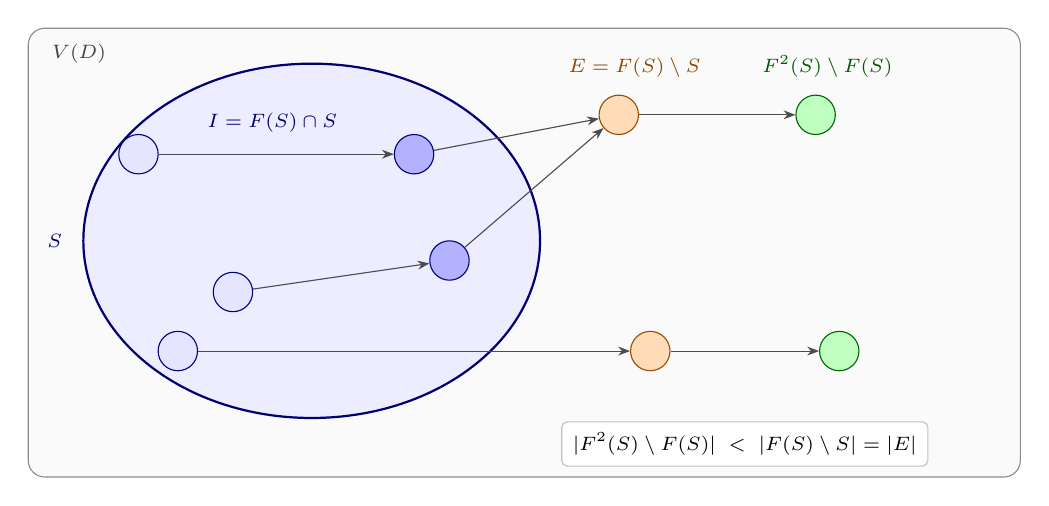
\begin{tikzpicture}[
  svert/.style={circle,draw=blue!50!black,fill=blue!10,inner sep=0pt,minimum size=5mm,font=\scriptsize},
  ivert/.style={circle,draw=blue!50!black,fill=blue!30,inner sep=0pt,minimum size=5mm,font=\scriptsize},
  evert/.style={circle,draw=orange!60!black,fill=orange!28,inner sep=0pt,minimum size=5mm,font=\scriptsize},
  gvert/.style={circle,draw=green!40!black,fill=green!25,inner sep=0pt,minimum size=5mm,font=\scriptsize},
  arc/.style={-{Stealth[length=1.5mm]},draw=black!70},
  lab/.style={font=\scriptsize,text=black!75}
]
% ambient box
\draw[draw=black!45,rounded corners=6pt,fill=black!2] (0,0) rectangle (12.6,5.7);
\node[lab,anchor=north west] at (0.18,5.62) {$V(D)$};
% S
\draw[blue!45!black,fill=blue!7,thick] (3.6,3.0) ellipse (2.9 and 2.25);
\node[lab,text=blue!45!black,anchor=west] at (0.12,3.0) {$S$};
% vertices
\node[svert] (s1) at (1.4,4.1) {};
\node[svert] (s2) at (1.9,1.6) {};
\node[svert] (s3) at (2.6,2.35) {};
\node[ivert] (i1) at (4.9,4.1) {};
\node[ivert] (i2) at (5.35,2.75) {};
\node[evert] (e1) at (7.5,4.6) {};
\node[evert] (e2) at (7.9,1.6) {};
\node[gvert] (g1) at (10.0,4.6) {};
\node[gvert] (g2) at (10.3,1.6) {};
% arcs
\draw[arc] (s1) -- (i1);
\draw[arc] (s3) -- (i2);
\draw[arc] (i2) -- (e1);
\draw[arc] (i1) -- (e1);
\draw[arc] (e1) -- (g1);
\draw[arc] (s2) -- (e2);
\draw[arc] (e2) -- (g2);
% region labels, all clear of nodes and arcs
\node[lab,text=blue!45!black,anchor=south] at (3.1,4.25) {$I=F(S)\cap S$};
\node[lab,text=orange!55!black,anchor=south] at (7.7,4.95) {$E=F(S)\setminus S$};
\node[lab,text=green!35!black,anchor=south] at (10.15,4.95) {$F^2(S)\setminus F(S)$};
% the inequality, on a plate below the ellipse
\node[draw=black!25,fill=white,rounded corners=2pt,inner sep=4pt,font=\scriptsize]
  at (9.1,0.42) {$\abs{F^2(S)\setminus F(S)} \;<\; \abs{F(S)\setminus S}=\abs E$};
\end{tikzpicture}
}
  \end{column}
  \end{columns}
  \takeaway{The right-hand side is the \emph{external} part of the first image only; that
  refinement is what the last step of the proof needs.}
\end{frame}

\begin{frame}{How the deficit is proved}
  \small
  Fix $S$. For $Y\subsetneq E$, delete \emph{all} arcs from $S$ to $E\setminus Y$:
  \begin{itemize}
    \item the graph $D_Y$ has fewer arcs, so minimality gives a vertex $v$ with
      $\abs{N_{1,D_Y}^+(v)}\le\abs{N_{2,D_Y}^+(v)}$;
    \item so $v\in S$, and $Q_v=F(\{v\})\cap(E\setminus Y)$ are the out-neighbors it loses.
  \end{itemize}
  \medskip
  \centering
  \scalebox{0.60}{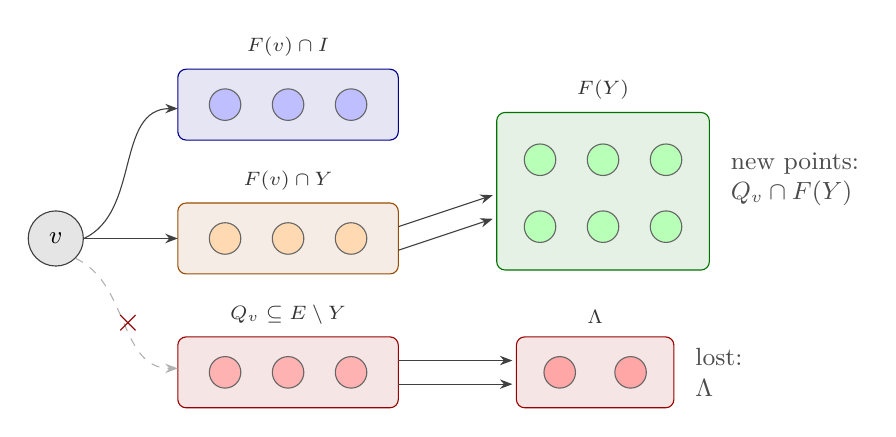
\begin{tikzpicture}[
  dot/.style={circle,draw=black!60,fill=#1,inner sep=0pt,minimum size=4mm},
  dot/.default=black!10,
  grp/.style={draw=#1,fill=#1!10,rounded corners=3pt},
  grp/.default=black!40,
  arc/.style={-{Stealth[length=1.6mm]},draw=black!75},
  del/.style={-{Stealth[length=1.6mm]},draw=black!30,dashed},
  lab/.style={font=\scriptsize,text=black!80},
  annot/.style={font=\small,text=black!70,align=left}
]
% v
\node[circle,draw=black!75,fill=black!10,inner sep=0pt,minimum size=7mm,font=\small] (v) at (0.7,2.8) {$v$};
% three groups of out-neighbours (drawn as boxes, labels above)
\draw[grp=blue!55!black] (2.25,4.05) rectangle (5.05,4.95);
\node[lab,anchor=south] at (3.65,4.99) {$F(v)\cap I$};
\node[dot=blue!25] at (2.85,4.5) {}; \node[dot=blue!25] at (3.65,4.5) {}; \node[dot=blue!25] at (4.45,4.5) {};
\draw[grp=orange!60!black] (2.25,2.35) rectangle (5.05,3.25);
\node[lab,anchor=south] at (3.65,3.29) {$F(v)\cap Y$};
\node[dot=orange!30] at (2.85,2.8) {}; \node[dot=orange!30] at (3.65,2.8) {}; \node[dot=orange!30] at (4.45,2.8) {};
\draw[grp=red!60!black] (2.25,0.65) rectangle (5.05,1.55);
\node[lab,anchor=south] at (3.65,1.59) {$Q_v\subseteq E\setminus Y$};
\node[dot=red!30] at (2.85,1.1) {}; \node[dot=red!30] at (3.65,1.1) {}; \node[dot=red!30] at (4.45,1.1) {};
% kept and deleted arcs out of v
\draw[arc] (v.east) to[out=25,in=180] (2.25,4.45);
\draw[arc] (v.east) to[out=0,in=180]  (2.25,2.8);
\draw[del] (v.south east) to[out=-25,in=180] (2.25,1.15);
\node[font=\large,text=red!55!black] at (1.62,1.72) {$\times$};
% F(Y) and Lambda
\draw[grp=green!45!black] (6.3,2.4) rectangle (9.0,4.4);
\node[lab,anchor=south] at (7.65,4.44) {$F(Y)$};
\node[dot=green!28] at (6.85,3.8) {}; \node[dot=green!28] at (7.65,3.8) {}; \node[dot=green!28] at (8.45,3.8) {};
\node[dot=green!28] at (6.85,2.95) {}; \node[dot=green!28] at (7.65,2.95) {}; \node[dot=green!28] at (8.45,2.95) {};
\draw[grp=red!60!black] (6.55,0.65) rectangle (8.55,1.55);
\node[lab,anchor=south] at (7.55,1.59) {$\Lambda$};
\node[dot=red!35] at (7.1,1.1) {}; \node[dot=red!35] at (8.0,1.1) {};
% arcs into F(Y) and Lambda
\draw[arc] (5.05,2.95) -- (6.25,3.35);
\draw[arc] (5.05,2.65) -- (6.25,3.05);
\draw[arc] (5.05,1.25) -- (6.5,1.25);
\draw[arc] (5.05,0.95) -- (6.5,0.95);
% side annotations
\node[annot,anchor=west] at (9.15,3.55) {new points:\\ $Q_v\cap F(Y)$};
\node[annot,anchor=west] at (8.7,1.1) {lost:\\ $\Lambda$};
\end{tikzpicture}
}
  \takeaway{The second out-neighborhood loses $\Lambda$ and gains only points of $Q_v\cap F(Y)$,
  which are \emph{first} out-neighbors: the gain is paid for out of the loss.}
\end{frame}

\begin{frame}{The ledger, and why the gain is strict}
  \small
  At the chosen vertex $v$, with $d_1=\abs{N_1^+(v)}$, $d_2=\abs{N_2^+(v)}$ in $D$:
  \begin{center}
  \renewcommand{\arraystretch}{1.25}
  \begin{tabular}{@{}llll@{}}
  \toprule
  quantity & in $D$ & in $D_Y$ & why \\
  \midrule
  $\abs{N_1^+(v)}$ & $d_1$ & $d_1-\abs{Q_v}$ & exactly $Q_v$ is lost \\
  $\abs{N_2^+(v)}$ & $d_2$ & $\le d_2-\abs\Lambda+\abs{Q_v\cap F(Y)}$ & $\Lambda$ destroyed, new points only here \\
  $g(Y)=\abs{F(Y)\setminus(I\cup Y)}$ & $g(Y)$ & $g(Y)+\abs\Lambda-\abs{Q_v\cap F(Y)}$ & exact \\
  \bottomrule
  \end{tabular}
  \end{center}
  \medskip
  The inequality at $v$ in $D_Y$ gives
  \[
    \abs\Lambda-\abs{Q_v\cap F(Y)}=g(Y\cup Q_v)-g(Y)\le\abs{Q_v}+d_2-d_1<\abs{Q_v},
  \]
  the last step because $D$ is a counterexample. Summing from $Y=\varnothing$ to $Y=E$:
  $g(E)<\abs E$, which is the lemma.
  \takeaway{Strictness comes from $d_2<d_1$; the deletion only has to \emph{pay} for what it
  gains.}
\end{frame}

\begin{frame}{Engine 1b: the blowup}
  \small
  The deficit is an integer, so it is at least $1$. Amplify it: replace every vertex by a
  transitive tournament on $m$ labels, and put all arcs from block $v$ to block $w$ when
  $v\to w$.
  \medskip

  \centering
  \scalebox{0.72}{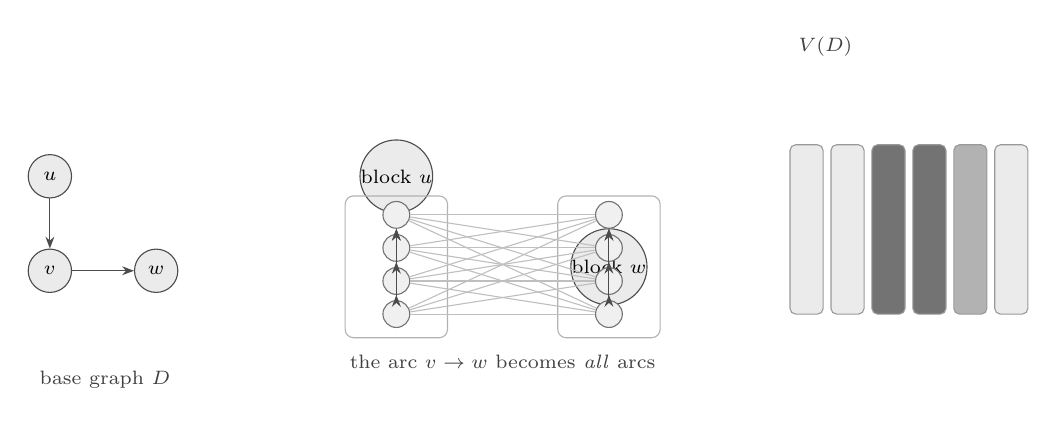
\begin{tikzpicture}[
  base/.style={circle,draw=black!70,fill=black!8,inner sep=0pt,minimum size=5.5mm,font=\scriptsize},
  labd/.style={circle,draw=black!55,fill=black!6,inner sep=0pt,minimum size=3.4mm},
  arc/.style={-{Stealth[length=1.5mm]},draw=black!70},
  thickarc/.style={-{Stealth[length=2.4mm]},draw=black!80,line width=1.4pt},
  lab/.style={font=\scriptsize,text=black!75},
  panel/.style={font=\scriptsize\bfseries,text=black!55}
]
% ---------------- panel 1: base graph
\begin{scope}
\node[base] (u) at (0,2.2) {$u$};
\node[base] (v) at (0,1.0) {$v$};
\node[base] (w) at (1.35,1.0) {$w$};
\draw[arc] (u) -- (v);
\draw[arc] (v) -- (w);
\node[lab,anchor=north] at (0.7,-0.15) {base graph $D$};
\end{scope}
% ---------------- panel 2: blowup of one arc
\begin{scope}[shift={(4.2,0)}]
\node[base,minimum size=6mm] (U) at (0.2,2.2) {block $u$};
\draw[rounded corners=3pt,draw=black!30] (-0.45,0.15) rectangle (0.85,1.95);
\node[base,minimum size=6mm] (W) at (2.9,1.05) {block $w$};
\draw[rounded corners=3pt,draw=black!30] (2.25,0.15) rectangle (3.55,1.95);
% block u: 4 labels
\foreach \i in {0,1,2,3}{
  \node[labd] (a\i) at (0.2,0.45+\i*0.42) {};
}
\draw[arc] (a0) -- (a1); \draw[arc] (a1) -- (a2); \draw[arc] (a2) -- (a3);
\draw[arc] (a0) -- (a3);
\foreach \i in {0,1,2,3}{
  \node[labd] (b\i) at (2.9,0.45+\i*0.42) {};
}
\draw[arc] (b0) -- (b1); \draw[arc] (b1) -- (b2); \draw[arc] (b2) -- (b3);
\draw[arc] (b0) -- (b3);
% complete bipartite
\foreach \i in {0,1,2,3}{ \foreach \j in {0,1,2,3}{ \draw[black!25] (a\i) -- (b\j); }}
\node[lab,anchor=north] at (1.55,0.05) {the arc $v\to w$ becomes \emph{all} arcs};
\end{scope}
% ---------------- panel 3: block classification
\begin{scope}[shift={(9.4,0)}]
\node[lab,anchor=south] at (0.45,3.6) {$V(D)$};
\foreach \k/\c in {0/black!8, 1/black!8, 2/black!55, 3/black!55, 4/black!30, 5/black!8}{
  \draw[rounded corners=2pt,draw=black!40,fill=\c] (\k*0.52,0.45) rectangle (\k*0.52+0.42,2.6);
}

\end{scope}
\end{tikzpicture}
}
  \medskip

  \raggedright
  For $U$ meeting the blocks in $S$: blocks of $F(S)$ are \emph{full} in $F_G(U)$, blocks of
  $F^2(S)$ are full in $F_G^2(U)$, and inside a partly used block the internal defect is at most
  one label. Hence, with $n$ blocks,
  \[
    \abs U-2\abs{F_G(U)}+\abs{F_G^2(U)}
    \le m\underbrace{\bigl(\abs{F^2(S)\setminus F(S)}-\abs{F(S)\setminus S}\bigr)}_{\le-1}+n<0
    \qquad\text{once } m\ge n .
  \]
  \takeaway{A margin of one becomes a margin of $m$, which beats the bounded defect $n$.}
\end{frame}

\begin{frame}{The object we now have to destroy}
  \begin{block}{Proposition 4.1 (to be contradicted)}
    There is \textbf{no} nonempty finite oriented graph $G$ with all indegrees positive and
    \[
      \abs U+\abs{F^2(U)}<2\abs{F(U)}\qquad\text{for every nonempty proper }U .
    \]
  \end{block}
  \medskip
  \small
  So from now on $G$ is such a graph, $X=V(G)$, and the only input is the display above.
  \medskip

  \begin{itemize}
    \item The hypothesis is about \emph{sets of vertices}.
    \item Families of ordered pairs have columns and rows that \emph{are} sets of vertices.
    \item So: apply the hypothesis to columns and rows, and sum.
  \end{itemize}
  \takeaway{The passage from vertices to \emph{pairs of vertices} is what makes the inequality
  usable: a family of pairs has many columns and rows at once.}
\end{frame}

\begin{frame}{Engine 2: two families of pairs}
  \small
  For $P,Q\subseteq X\times X$:
  \[
    \Phi_1P=\{(i,j):(p,j)\in P,\ p\to i\},\qquad
    \Phi_2Q=\{(i,j):(i,s)\in Q,\ s\to j\}.
  \]
  $P,Q$ are \emph{compatible} if $\Phi_1P\cap\Phi_2Q=\varnothing$. A conflicting pair produces a
  rectangle:
  \medskip
  \centering
  \scalebox{0.66}{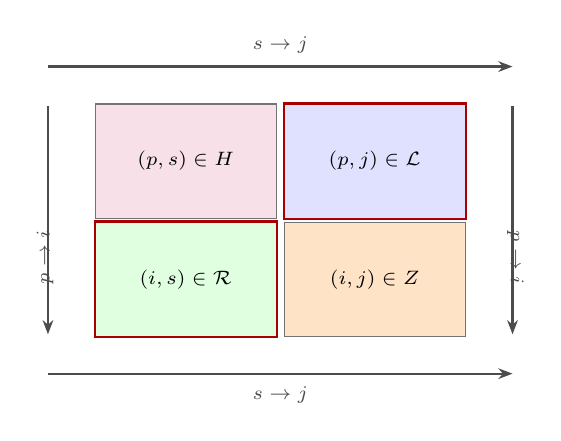
\begin{tikzpicture}[
  cell/.style={draw=black!55,minimum width=2.3cm,minimum height=1.45cm,align=center,
               font=\scriptsize,inner sep=2pt},
  hcell/.style={cell,fill=purple!12},
  lcell/.style={cell,fill=blue!12},
  rcell/.style={cell,fill=green!12},
  zcell/.style={cell,fill=orange!22},
  trav/.style={-{Stealth[length=1.8mm]},draw=black!70,thick},
  lab/.style={font=\scriptsize,text=black!70}
]
% the four cells: row p (top), row i (bottom); column s (left), column j (right)
\node[hcell] (ps) at (-1.2,0.75) {$(p,s)\in H$};
\node[lcell] (pj) at (1.2,0.75) {$(p,j)\in\mathcal L$};
\node[rcell] (is) at (-1.2,-0.75) {$(i,s)\in\mathcal R$};
\node[zcell] (ij) at (1.2,-0.75) {$(i,j)\in Z$};
% the conflicting pair: thick red border
\draw[red!65!black,thick] (pj.north west) rectangle (pj.south east);
\draw[red!65!black,thick] (is.north west) rectangle (is.south east);
% the square of traversals, outside the block
\draw[trav] (-2.95,1.45) -- (-2.95,-1.45) node[midway,left=1pt,lab,rotate=90] {$p\to i$};
\draw[trav] (-2.95,1.95) -- (2.95,1.95) node[midway,above=1pt,lab] {$s\to j$};
\draw[trav] (2.95,1.45) -- (2.95,-1.45) node[midway,right=1pt,lab,rotate=-90] {$p\to i$};
\draw[trav] (-2.95,-1.95) -- (2.95,-1.95) node[midway,below=1pt,lab] {$s\to j$};
\end{tikzpicture}
}
  \takeaway{Columns of $P$ and rows of $Q$ are vertex sets, so the hypothesis applies to them; and
  compatibility is exactly what makes the uncovered points countable.}
\end{frame}

\begin{frame}{The extremal objective}
  \small
  \begin{block}{Choose $(P,Q)$}
    compatible, containing the diagonal $\Delta=\{(v,v)\}$, maximising
    \[
      M+u,\qquad M=\abs P+\abs Q,\qquad
      u=\abs{X^2}-\abs{\Phi_1P}-\abs{\Phi_2Q}\ \text{(uncovered points)}.
    \]
  \end{block}
  \medskip
  Why $+u$ and not just $M$?
  \begin{itemize}
    \item Summing the hypothesis over the columns of $P$ and the rows of $Q$ gives
      $\abs P+\abs{\Phi_1^2P}<2\abs{\Phi_1P}$ and the same for $Q$;
    \item taking complements $\mathcal L=X^2\setminus\Phi_2^2Q$,
      $\mathcal R=X^2\setminus\Phi_1^2P$ then gives
      \[
        \abs{\mathcal L}+\abs{\mathcal R}>M+2u :
      \]
      \textbf{two copies of the uncovered count}, one from each inequality.
    \item The pruning will cost at most $u+u'$ and refund $u'$; so the objective $M+u$ is exactly
      what survives.
  \end{itemize}
  \takeaway{The factor $2$ in the gain is why the objective carries $u$: one copy pays the
  collisions, one copy is refunded.}
\end{frame}

\begin{frame}{The diagonal survives}
  \small
  $\mathcal L,\mathcal R$ may conflict, but the diagonal does not:
  \medskip
  \centering
  \scalebox{0.8}{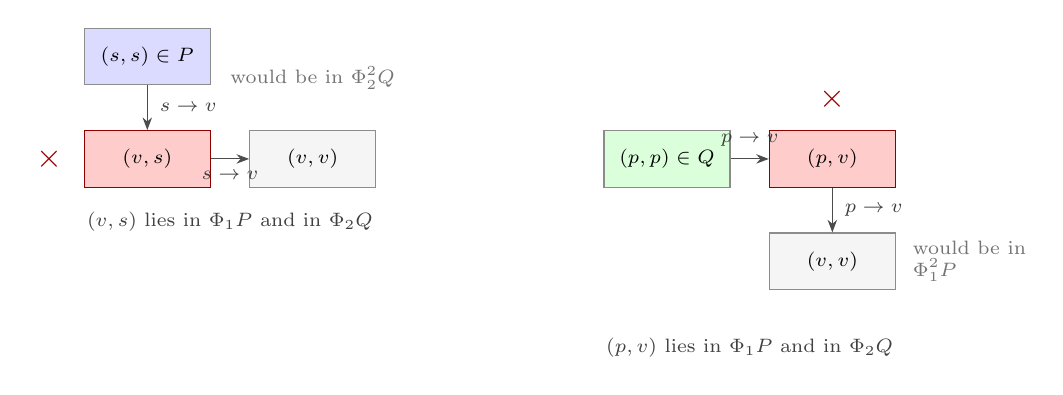
\begin{tikzpicture}[
  cell/.style={draw=black!45,minimum width=1.6cm,minimum height=0.72cm,align=center,
               font=\scriptsize,inner sep=1pt},
  pc/.style={cell,fill=blue!14},
  qc/.style={cell,fill=green!14},
  bad/.style={cell,fill=red!20,draw=red!55!black},
  neut/.style={cell,fill=black!4},
  ar/.style={-{Stealth[length=1.6mm]},draw=black!70},
  lab/.style={font=\scriptsize,text=black!75}
]
% ---- case 1: (v,v) not in Phi_2^2 Q
\node[pc]   (ss) at (0,1.3) {$(s,s)\in P$};
\node[bad]  (vs) at (0,0)   {$(v,s)$};
\node[neut] (vv) at (2.1,0) {$(v,v)$};
\draw[ar] (ss) -- node[right=1pt,lab] {$s\to v$} (vs);
\draw[ar] (vs) -- node[below=1pt,lab] {$s\to v$} (vv);
\node[font=\large,text=red!60!black,anchor=east] at (-0.95,0) {$\times$};
\node[lab,anchor=north,align=center] at (1.05,-0.55) {$(v,s)$ lies in $\Phi_1P$ and in $\Phi_2Q$};
\node[lab,anchor=north,align=center,text=black!55] at (2.1,1.3) {would be in $\Phi_2^2Q$};
% ---- case 2: (v,v) not in Phi_1^2 P
\node[qc]   (pp) at (6.6,0)   {$(p,p)\in Q$};
\node[bad]  (pv) at (8.7,0)   {$(p,v)$};
\node[neut] (vv2) at (8.7,-1.3) {$(v,v)$};
\draw[ar] (pp) -- node[above=1pt,lab] {$p\to v$} (pv);
\draw[ar] (pv) -- node[right=1pt,lab] {$p\to v$} (vv2);
\node[font=\large,text=red!60!black,anchor=south] at (8.7,0.5) {$\times$};
\node[lab,anchor=north,align=center] at (7.65,-2.15) {$(p,v)$ lies in $\Phi_1P$ and in $\Phi_2Q$};
\node[lab,anchor=west,align=left,text=black!55] at (9.6,-1.3) {would be in\\ $\Phi_1^2P$};
\end{tikzpicture}
}
  \medskip

  If $(v,v)\in\Phi_2^2Q$, then $(v,s)\in\Phi_2Q$ for some $s\to v$; but $(s,s)\in P$ and $s\to v$
  give $(v,s)\in\Phi_1P$, contradicting compatibility. Symmetrically for $\Phi_1^2P$.
  \takeaway{The diagonal is admissible, survives the complement, and is conflict-free: it is the
  seed that makes the pruned pair a legitimate competitor.}
\end{frame}

\begin{frame}{Engine 3: pruning}
  \begin{block}{Lemma (pruning; any finite binary relation)}
    For families $\mathcal L,\mathcal R\subseteq X\times X$ there are
    $\mathcal L'\subseteq\mathcal L$, $\mathcal R'\subseteq\mathcal R$ with no conflicts, keeping
    every initially conflict-free member, and
    \[
      \abs{\mathcal L\setminus\mathcal L'}+\abs{\mathcal R\setminus\mathcal R'}
      \le\abs H+\#\{z\in Z:\ z\text{ uncovered by }\mathcal L'\cup\mathcal R'\},
    \]
    where $Z$ = conflict points, $H$ = collisions.
  \end{block}
  \small
  \medskip
  \begin{columns}
  \begin{column}{0.5\textwidth}
    \centering
    \scalebox{0.72}{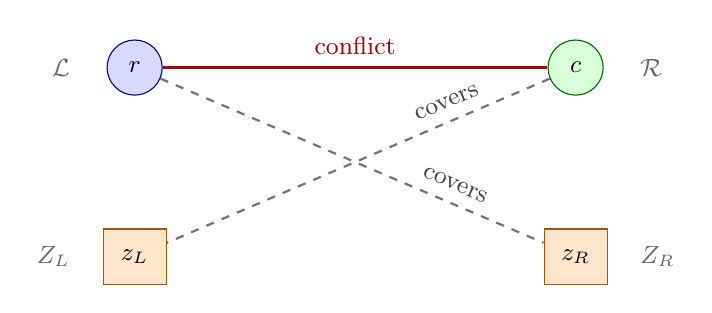
\begin{tikzpicture}[
  lv/.style={circle,draw=blue!55!black,fill=blue!15,minimum size=7mm,inner sep=0pt,font=\small},
  rv/.style={circle,draw=green!40!black,fill=green!15,minimum size=7mm,inner sep=0pt,font=\small},
  zv/.style={rectangle,draw=orange!65!black,fill=orange!20,minimum width=8mm,minimum height=7mm,inner sep=1pt,font=\small},
  conf/.style={draw=red!65!black,thick,line width=1pt},
  cov/.style={draw=black!55,dashed,thick},
  lab/.style={font=\small,text=black!75},
  grp/.style={font=\small\bfseries,text=black!60}
]
\node[lv] (r) at (0,2.6) {$r$};
\node[zv] (zl) at (0,0.2) {$z_L$};
\node[rv] (c) at (5.6,2.6) {$c$};
\node[zv] (zr) at (5.6,0.2) {$z_R$};
\node[grp,anchor=east] at (-0.7,2.6) {$\mathcal L$};
\node[grp,anchor=east] at (-0.7,0.2) {$Z_L$};
\node[grp,anchor=west] at (6.3,2.6) {$\mathcal R$};
\node[grp,anchor=west] at (6.3,0.2) {$Z_R$};
\draw[conf] (r) -- node[above=1pt,lab,text=red!60!black] {conflict} (c);
\draw[cov] (c) -- node[above=1pt,lab,sloped,near start] {covers} (zl);
\draw[cov] (r) -- node[above=1pt,lab,sloped,near end] {covers} (zr);
\end{tikzpicture}
}
  \end{column}
  \begin{column}{0.50\textwidth}
    \footnotesize
    Conflicts and covering relations become edges of one bipartite graph $\Gamma$.
    A vertex cover of size $\abs Z+\abs H$ gives the bound:
    each of the $\abs Z-q$ covered conflict points needs its own copy in the cover.
  \end{column}
  \end{columns}
  \takeaway{Two families that are almost compatible are made compatible, at a cost charged to the
  collisions and to the points left uncovered.}
\end{frame}

\begin{frame}{How the pruning is proved}
  \small
  It suffices to bound a maximum matching $\mathcal M$ of $\Gamma$ by $\abs Z+\abs H$. Split it:
  \[
    \abs{\mathcal M}=k+\ell+t,
  \]
  $k$ edges between original members, $\ell$ between $\mathcal L$ and $Z_R$ (a maximum matching
  $\alpha$), $t$ between $Z_L$ and $\mathcal R$ (a maximum matching $\beta$).
  \medskip
  \begin{columns}
  \begin{column}{0.50\textwidth}
    \centering
    \scalebox{0.78}{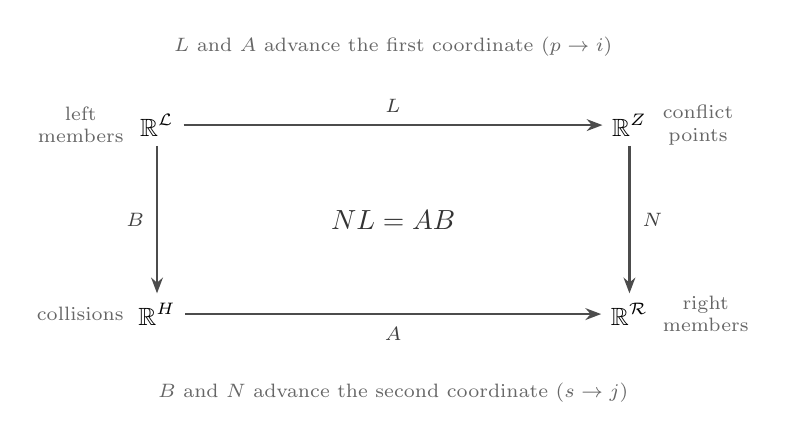
\begin{tikzpicture}[
  sp/.style={font=\small},
  ar/.style={-{Stealth[length=2mm]},draw=black!70,thick},
  lab/.style={font=\scriptsize,text=black!75},
  note/.style={font=\scriptsize,text=black!60,align=center}
]
\node[sp] (L) at (0,2.4) {$\R^{\mathcal L}$};
\node[sp] (Z) at (6.0,2.4) {$\R^{Z}$};
\node[sp] (H) at (0,0) {$\R^{H}$};
\node[sp] (R) at (6.0,0) {$\R^{\mathcal R}$};
\draw[ar] (L) -- node[above=1pt,lab] {$L$} (Z);
\draw[ar] (L) -- node[left=1pt,lab] {$B$} (H);
\draw[ar] (H) -- node[below=1pt,lab] {$A$} (R);
\draw[ar] (Z) -- node[right=1pt,lab] {$N$} (R);
\node[lab,text=black!80,font=\normalsize] at (3.0,1.2) {$NL=AB$};
\node[note,anchor=east] at (-0.3,2.4) {left\\ members};
\node[note,anchor=west] at (6.3,2.4) {conflict\\ points};
\node[note,anchor=east] at (-0.3,0) {collisions};
\node[note,anchor=west] at (6.3,0) {right\\ members};
\node[note,anchor=south] at (3.0,3.15) {$L$ and $A$ advance the first coordinate ($p\to i$)};
\node[note,anchor=north] at (3.0,-0.75) {$B$ and $N$ advance the second coordinate ($s\to j$)};
\end{tikzpicture}
}
  \end{column}
  \begin{column}{0.42\textwidth}
    \footnotesize
    Two independent arrays $a_{xy}$, $b_{xy}$ of variables. Four matrices $L,N,A,B$; changing the
    two coordinates in opposite orders gives the same entry:
    \[ NL=AB. \]
    Choose the coefficients so that $\rank L=\ell$, $\rank N^{\mathsf T}=t$, and so that some
    auxiliary matrices achieve maximum rank.
  \end{column}
  \end{columns}
  \takeaway{Three parts, each counted by a rank; the commuting square forces the $k$
  original--original edges into $\ker A$.}
\end{frame}

\begin{frame}{The rank bookkeeping, in one line}
  \small
  From $NL=AB$ we get $\im(NL)\subseteq\im A$; by rank--nullity
  $\dim\ker A=\abs H-\rank A$. Hence
  \[
    \abs H=\dim\ker A+\rank A
    \;\ge\; k+\rank(NL)
    \;\ge\; k+\ell-(\abs Z-t)
    \;=\;k+\ell+t-\abs Z .
  \]
  So it remains to show $\dim\ker A\ge k$.
  \medskip

  \begin{block}{The lift}
    For each original--original edge $r=(p,j)$ find $\lambda^r\in\ker L$ with $\lambda^r_r=1$ and
    $\lambda^r_{r'}=0$ for the other original left endpoints. Then $B\lambda^r\in\ker A$, and
    \[
      \sum_r\theta_r B\lambda^r=0\ \Longrightarrow\ u=\sum_r\theta_r\lambda^r\in\ker B,\quad
      u_r=\theta_r=0 .
    \]
  \end{block}
  \takeaway{The key vanishing $u_{pj}v_{is}=0$ at conflicts (proved by the maximum-rank lemma)
  makes the right kernel vector kill each coordinate, so the $k$ lifts survive.}
\end{frame}

\begin{frame}{The contradiction}
  \small
  \begin{columns}[T]
  \begin{column}{0.52\textwidth}
    Apply pruning to $\mathcal L,\mathcal R$, keeping $\Delta$:
    \begin{itemize}
      \item at most $\abs H+q\le u+u'$ members are deleted;
      \item the survivors are compatible, contain $\Delta$, and are worth
        \[
          \abs{\mathcal L'}+\abs{\mathcal R'}+u'
          \ge\abs{\mathcal L}+\abs{\mathcal R}-u>M+u ;
        \]
      \item but $(P,Q)$ maximised $M+u$ among admissible pairs. Contradiction.
    \end{itemize}
    \medskip
    So no graph with all indegrees positive satisfies the strict inequality, and
    Proposition 2.1 produced one. The theorem follows.
  \end{column}
  \begin{column}{0.50\textwidth}
    \centering
    \scalebox{0.85}{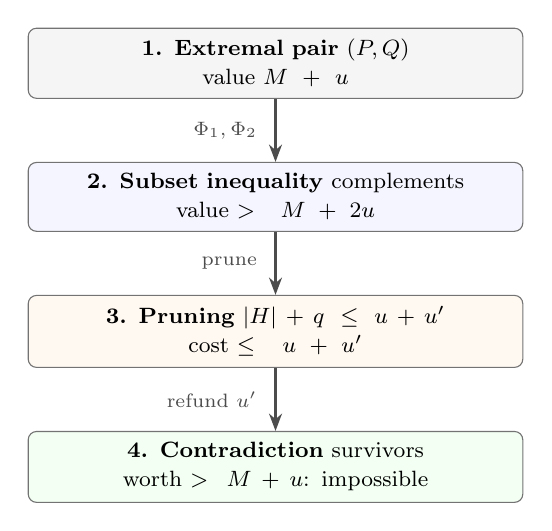
\begin{tikzpicture}[
  stage/.style={draw=black!55,rounded corners=3pt,align=center,font=\footnotesize,
                inner sep=4pt,text width=6.0cm,fill=#1},
  stage/.default=white,
  ar/.style={-{Stealth[length=2.2mm]},draw=black!70,thick},
  lab/.style={font=\scriptsize,text=black!70,align=left}
]
\node[stage=black!4] (s1) at (0,0) {\textbf{1. Extremal pair} $(P,Q)$\\[1pt] value $M+u$};
\node[stage=blue!4,below=8mm of s1] (s2) {\textbf{2. Subset inequality} complements\\[1pt] value $>M+2u$};
\node[stage=orange!5,below=8mm of s2] (s3) {\textbf{3. Pruning} $\abs H+q\le u+u'$\\[1pt] cost $\le u+u'$};
\node[stage=green!5,below=8mm of s3] (s4) {\textbf{4. Contradiction} survivors\\[1pt] worth $>M+u$: impossible};
\draw[ar] (s1.south) -- node[left=3pt,lab] {$\Phi_1,\Phi_2$} (s2.north);
\draw[ar] (s2.south) -- node[left=3pt,lab] {prune} (s3.north);
\draw[ar] (s3.south) -- node[left=3pt,lab] {refund $u'$} (s4.north);
\end{tikzpicture}
}
  \end{column}
  \end{columns}
  \takeaway{$\abs{\mathcal L}+\abs{\mathcal R}>M+2u$ minus the cost $u+u'$ plus the refund $u'$
  beats $M+u$: there is no such graph.}
\end{frame}

\begin{frame}{Consequences}
  \small
  \begin{itemize}
    \item \textbf{Weighted forms} (Seacrest): for every vertex weighting there is a good vertex;
      there is a weighting of total mass $1$ for which every vertex is good; and the arc-weighted
      form with $\beta_v^w(s)=\max(0,\max_u(w(us)-w(vs)))$.
    \item \textbf{Directed cycles}: without a directed triangle, $N_2^+(v)\subseteq\overline N(v)$
      (the non-neighbors), so some $v$ has
      \[ d^+(v)\le\abs{\overline N(v)},\qquad n-1\ge 2d^+(v)+d^-(v). \]
    \item Hence $\delta^+\ge n/3$ and $\delta^-\ge n/3$ force a directed triangle, and a regular
      oriented graph of directed girth four has $n\ge3r+1$.
  \end{itemize}
  \takeaway{These are corollaries, not inputs: the main theorem is proved before they appear.}
\end{frame}

\begin{frame}{Why the weight on uncovered points is exactly 1}
  \small
  Suppose the objective were $|P|+|Q|+\lambda u$ for some other $\lambda>0$. The ledger of the
  previous frame becomes
  \[
    \text{new value} > \underbrace{M+\lambda u}_{\text{old value}}+(\lambda-1)(u'-u).
  \]
  \medskip
  \begin{itemize}
    \item $\lambda=1$: the last term vanishes, the gain is the strict inequality, done.
    \item $\lambda<1$: the argument fails as soon as $u'>u$.
    \item $\lambda>1$: the argument fails as soon as $u'<u$.
  \end{itemize}
  \medskip
  Both cases occur, so no other weight works for all instances.
  \takeaway{the coefficient $1$ is forced by the shape of the pruning bound, not a lucky guess.}
\end{frame}

\begin{frame}{What does \emph{not} simplify}
  \small
  \begin{columns}[T]
  \begin{column}{0.49\textwidth}
    \textbf{Removed (this talk's rewriting)}
    \begin{itemize}
      \item Edmonds' rank formula: only the easy direction is used, and it is a determinant
        expansion.
      \item Seacrest's equivalence for the vertex-weighted forms: clusters of twins give (i),
        Farkas gives (ii).
      \item $m>n$: the blowup works with $m\ge n$.
    \end{itemize}
  \end{column}
  \begin{column}{0.49\textwidth}
    \textbf{Not removable}
    \begin{itemize}
      \item The blowup: the deficit holds at $S$ but concavity fails there, in a 4-vertex graph.
      \item The rank argument: a collision is shared by many conflicts, so no injection exists.
      \item The weight $1$: see the previous frame.
    \end{itemize}
  \end{column}
  \end{columns}
  \takeaway{the three engines are irremovable; what surrounds them can be made lighter.}
\end{frame}

\begin{frame}{The three inventions}
  \begin{enumerate}
    \item \textbf{A subset inequality with the right right-hand side.}
      $\abs{F^2(S)\setminus F(S)}<\abs{F(S)\setminus S}$: the external part of the first image,
      obtained by deleting arcs and buying second out-neighbors out of first ones.
    \item \textbf{Pruning at a cost charged to the survivors.}
      Two almost-compatible families become compatible; the price is the collisions plus the
      conflict points left uncovered.
    \item \textbf{An extremal objective that refunds the cost.}
      Maximise $M+u$; the subset inequality gives $M+2u$, pruning costs $u+u'$ and refunds $u'$.
  \end{enumerate}
  \medskip
  \begin{block}{The single idea behind all three}
    Never compare a set with itself: compare it with what it \emph{produces} and what it
    \emph{costs}, and let the two cancelling terms be the same quantity counted twice.
  \end{block}
  \takeaway{Everything else in the paper is a definition, a standard consequence, or bookkeeping.}
\end{frame}

\begin{frame}{Summary}
  \small
  \begin{itemize}
    \item Seymour's second-neighborhood conjecture is true for all oriented graphs.
    \item The proof is a reduction to an extremal statement about two families of ordered pairs,
      plus a linear-algebraic pruning lemma for arbitrary finite relations.
    \item The three engines are independent: the reduction uses minimality and a blowup; the
      pruning lemma uses matrix ranks and K\H{o}nig's theorem; the extremal argument uses an
      objective designed so that the pruning cost cancels.
    \item The weighted and directed-cycle consequences follow from Seacrest's equivalences and from
      one observation about triangles.
  \end{itemize}
  \vfill
  \begin{center}\small\color{mainblue}
    thank you --- questions?
  \end{center}
\end{frame}

\end{document}
